\chapter{CONVENȚII DE REDACTARE}

În această secțiune sunt detaliate convențiile de urmat în timpul editării lucrării.

\section{Cerințe generale}

Cerințele generale sunt preluate din [Olt07] (lucrare pe care o recomandăm călduros spre citire candidaților 
noștri, înainte de demararea redactării tezei): ,,responsabilitatea tezei este în întregime a candidatului, atât 
în ceea ce priveşte conţinutul, cât şi forma. Lucrarea trebuie să aibă o organizare clară şi riguroasă, care să 
dovedească gândirea inginerească a candidatului. Ideile exprimate în lucrare trebuie să se înlănţuie conform unei 
logici clare. În acest sens, elementele de coerenţă şi de coeziune a textului trebuie folosite în mod corect. Ideile 
se organizează în paragrafe, redactate cu indentaţie şi fără spaţiu între ele. Nu fraza creează paragraful, ci ideea!\\~\\

Stilul este extrem de important (,,Stilul este veşmântul gândului,'' spune Samuel Johnson). Lucrarea trebuie redactată 
într-un limbaj ştiinţific adecvat domeniului de cercetare abordat. Se vor evita particularităţile limbajului colocvial. 
Nu sunt admise greşeli gramaticale de redactare (acord, punctuaţie, lexic etc.). Lucrarea normativă ce va fi avută în vedere 
în această privinţă este Dicţionarul ortografic, ortoepic şi morfologic al limbii române [DOOM05].\\~\\

Candidatul are obligaţia de a verifica dacă datele, termenii folosiţi, numele proprii, citatele, titlurile (în limba 
română şi în alte limbi) sunt corecte. \\~\\

Candidatul trebuie să fie consecvent în exprimarea ideilor, în folosirea termenilor, a numelor proprii, a datelor, precum 
şi a punctuaţiei şi a elementelor de structură a lucrării. Consecvenţa este necesară şi în privinţa tipurilor de evidenţieri 
grafice folosite (litere cursive, litere îngroșate sau sublinieri).\\~\\

Termenii tehnici de origine străină neadaptaţi, consacraţi de lucrările de specialitate, nu se traduc, dar, dacă folosiţi 
o sursă bibliografică străină, puteţi încerca traducerea unor termeni noi, cu condiţia ca cei din limba de origine să fie 
prezenţi alături. În ambele cazuri, se recomandă scrierea acestor termeni cu litere speciale (de regulă italice). \\~\\

La cele menţionate mai sus, adăugăm următoarea observaţie, care nu este deloc lipsită de importanţă: notarea semnelor 
diacritice româneşti este obligatorie. Un text românesc în care ă se confundă cu a nu face o impresie bună, dă o notă 
de neglijenţă.”\\~\\

\section{Structura documentului}

Lucrarea trebuie să conțină următoarele capitole:

\begin{itemize}
    \item Coperta tezei;
    \item Pagina de titlu;
    \item Declarația de originalitate (completată și semnată de către autor);
    \item Formularul de înregistrare a enunțului temei lucrării (completat și semnat în solidar de către autor și coordonatorul științific);
    \item Referatul coordonatorului științific (completat și semnat de coordonator);
    \item Declarația de mulțumire a autorului (opțională);
    \item Cuprinsul lucrării;
    \item Lista figurilor;
    \item Lista tabelelor;
    \item Introducere;
    \item Conținutul propriu-zis al lucrării (capitolele constituente);
    \item Concluzii;
    \item Bibliografia;
    \item Referințele web;
    \item Anexele (index, codul sursă, site-ul web al aplicației, etc.).
\end{itemize}

\section{Dimensiunile lucrării}

Nu pot fi acceptate lucrări cu un număr de pagini mai mic decât 50. Prin urmare se dau, cu titlu de recomandare, 
următoarele dimensiuni:

\begin{itemize}
    \item 50 – 80 de pagini pentru o lucrare de licență;
    \item 60 – 100 de pagini pentru o lucrare de disertație.
\end{itemize}

În altă ordine de idei, recomandăm următoarea distribuție a paginilor pe diversele secțiuni/capitole [Olt07]:

\begin{itemize}
    \item Introducerea reprezintă cca. 10 – 15\% din lucrare;
    \item Conținutul reprezintă cca. 75 – 80\% din lucrare;
    \item Concluziile reprezintă cca. 10\%. 
\end{itemize}

\section{Elemente de tehnoredactare}

Pe scurt:

\begin{itemize}
    \item dimensiunea paginilor va fi A4, 21 x 29,7 cm; 
    \item marginile recomandate sunt: sus/jos/stânga/dreapta – 2,54 cm;
    \item fontul recomandat este Times New Roman; 
    \item corpul literelor va avea dimensiunea de 11 puncte;
    \item spațiul dintre rânduri va avea dimensiunea de 1 rând și jumătate (1,5); 
    \item indentarea unui paragraf se va face cu 1,27 cm;
    \item textul paragrafelor trebuie să fie aliniat în mod echilibrat stânga-dreapta (în eng. - justify);
    \item paginile trebuie să fie numerotate conform acestui șablon.
\end{itemize}

\section{Formulele matematice}

Pentru redactarea formulelor matematice recomandăm utilizarea instrumentului Microsoft 
Equation Editor și importul lor (o data terminate) în Microsoft Word.

\section{Ilustrațiile}

\subsection{Figurile}

Partea grafică a lucrării are o pondere semnificativă în nota finală acordată lucrării 
candidatului. Se recomandă prin urmare acordarea unei atenții sporite tehnoredactării figurilor.\\~\\
Actualizarea Listei Figurilor este obligatorie (procedura este similară cu cea exemplificată în secțiunea 2.5.2).

\subsection{Tabelele}

Exemplificăm aici utilizarea tabelor. Pentru fiecare tabelă adăugată lucrării, autorul trebuie să prevadă și adăugarea 
unei legende (în eng., Caption).  La final, este recomandată actualizarea listei figurilor. Pașii necesari pentru actualizarea 
listei tabelelor sunt:

\begin{enumerate}
    \item Click dreapta pe Lista Tabelelor. Va apărea un meniu similar cu cel din \autoref{fig:mesh1}
    
    \begin{figure}[h]
        \centering
        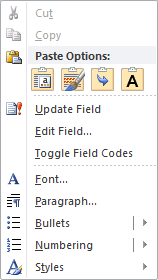
\includegraphics[width=0.20\textwidth]{meniu.png}
        \caption{Selectarea prin click dreapta a opțiunii ,,Update field''}
        \label{fig:mesh1}
    \end{figure}

    \item Selectarea opțiunii ,,Update entire tabl'' conform cu \autoref{fig:mesh2}
    \begin{figure}[h]
        \centering
        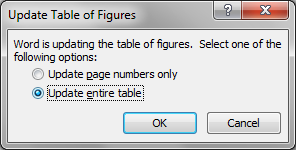
\includegraphics[width=0.35\textwidth]{meniu2.png}
        \caption{Actualizarea întregului tabel}
        \label{fig:mesh2}
    \end{figure}

    \item Verificarea fontului folosit pentru conținutul propriu-zis al Listei Tabelelor și alegerea 
    fontului Times New Roman în caz de incongruență.
    
    \begin{table}[h]
    \begin{center}
        \begin{tabular}{|c|c|c|}
            \hline\rowcolor[HTML]{f2f2f2}\textbf{Index} & \textbf{Nume utilizator} & \textbf{Valoarea rezumat a parolei (folosind SHA1)} \\\hline
            1 & dpopescu & 8fb9e6763269ae7cba85f02668c3c32041bf00ed \\\hline
            2 & eganea & 3b42ba8a586dd1589e949c28c9cf2810f7d65bb4 \\\hline
            3 & mmarian & bfc01d16d1944f3b6caba515556713f4aeeb2d0b \\\hline
        \end{tabular}
    \end{center}
    \caption{\label{tab:tabel1}\textbf{Nume de utilizatori și valorile rezumat ale parolelor acestora.}}
    \end{table}

\end{enumerate}

\newpage
În interiorul lucrării, tabelul poate fi citat folosind eticheta și numărul de ordine ale sale precum în 
exemplul acesta (vezi \autoref{tab:tabel1}). 

\subsection{Legenda (unei figuri/tabele)}
În cele doua secțiuni de mai sus s-au demonstrat două modele de legende atașate fiecărei tabele sau 
figuri. Microsoft Word permite modificarea, respectiv adăugarea de etichete noi corespunzătoare unui 
anumit tip de legendă. 